\documentclass[12pt]{article}
\usepackage[margin=2.5cm]{geometry}
\usepackage{enumerate}
\usepackage{amsfonts}
\usepackage{amsmath}
\usepackage{fancyhdr}
\usepackage{amsmath}
\usepackage{amssymb}
\usepackage{amsthm}
\usepackage{mdframed}
\usepackage{graphicx}
\usepackage{subcaption}
\usepackage{adjustbox}
\usepackage{listings}
\usepackage{xcolor}
\usepackage{booktabs}
\usepackage[utf]{kotex}
\usepackage{hyperref}

\definecolor{codegreen}{rgb}{0,0.6,0}
\definecolor{codegray}{rgb}{0.5,0.5,0.5}
\definecolor{codepurple}{rgb}{0.58,0,0.82}
\definecolor{backcolour}{rgb}{0.95,0.95,0.92}

\lstdefinestyle{mystyle}{
    backgroundcolor=\color{backcolour},
    commentstyle=\color{codegreen},
    keywordstyle=\color{magenta},
    numberstyle=\tiny\color{codegray},
    stringstyle=\color{codepurple},
    basicstyle=\ttfamily\footnotesize,
    breakatwhitespace=false,
    breaklines=true,
    captionpos=b,
    keepspaces=true,
    numbers=left,
    numbersep=5pt,
    showspaces=false,
    showstringspaces=false,
    showtabs=false,
    tabsize=1
}

\lstset{style=mystyle}

\pagestyle{fancy}
\renewcommand{\headrulewidth}{0.4pt}
\lhead{CSC 373}
\rhead{Worksheet 3 Solution}

\begin{document}
\title{CSC373 Worksheet 3 Solution}
\maketitle

\bigskip

\begin{enumerate}[1.]
    \item

    \bigskip

    \underline{\textbf{Notes:}}

    \bigskip

    \begin{itemize}
        \item Dynamic Programming

        \begin{itemize}
            \item Is applied to optimization problems
            \item Applies when the subproblems overlap
            \item Uses the following sequence of steps

            \begin{enumerate}[1.]
                \item Characterize the structure of an optimal solution
                \item Recursively define the value of an optimal solution
                \item Construct an optimal solution from computed information
            \end{enumerate}
        \end{itemize}

        \bigskip

        \item Matrix-chain Multiplication

        \begin{itemize}
            \item Is an optimization problem solved using dynamic programming
            \item Goal is to find matrix parenthesis with fewest number of operations

            \bigskip

            \underline{\textbf{Example:}}

            \bigskip

            Given chain of matrices $<A,B,C>$, it's fully parenthesized product is:

            \bigskip

            \begin{itemize}
                \item $(AB)C$ needs $(10 \times 30 \times 5) + (10 \times 5 \times 60) = 1500 + 3000 = 4500$ operations
                \item $A(BC)$ needs $(30 \times 5 \times 60) + (10 \times 30 \times 60) = 27000$ operations
            \end{itemize}

            \bigskip

            Thus, $(AB)C$ performs more efficiently than $A(BC)$.

            \bigskip

            \item Is stated as: given a chain $<A_1, A_2, ..., A_n>$ of $n$ matrices,
            where for $i = 1,2,...,n$ matrix $A_i$ has dimension $p_{i-1} \times p_i$,
            fully parenthesize the product $A_1A_2...A_n$ in a way that minimizes the number of scalar multiplications.

            \item Steps

            \begin{enumerate}[1.]
                \item \textbf{Check is the problem has Optimal Substructure}

                \bigskip

                Let us adopt the notation $A_{i...j}$ where $i \leq j$, for the matrix
                that results from evaluating the product $A_iA_{i+1}...A_j$.

                \bigskip

                Assume the solution has the following parentheses:

                \begin{align*}
                    (A_{i...k})(A_{k+1...j})
                \end{align*}

                \bigskip

                If there is a better way to multiply $(A_{i...k})$, then we
                would have a more optimal solution.

                \bigskip

                This would be a contradiction, as we already stated that we have the optimal
                solution for $A_{i...j}$.

                \bigskip

                Therefore, this problem has optimal substructure.

                \bigskip


                \item \textbf{Find the Recursive Solution}

                \bigskip

                Let $M[i,j]$ be the cost of multiplying matrices from $A_i$ to $A_j$

                \bigskip

                We want to find out at which $'k'$ returns the fewest number of multiplications,
                or the minimum number of $M$.

                \bigskip

                The recursive formula for the cost of multiplying from $A_i$ to $A_j$ is

                \begin{align}
                    M[i,j] = \begin{cases}
                        0 & \text{if $i = j$}\\
                        \min_{i \leq k \leq j} M[i,k] + M[k+1,j] + p_{i-1}p_{k}p_j & \text{if $i < j$}\\
                    \end{cases}
                \end{align}

                \item \textbf{Computing the Estimated Cost}
                \begin{itemize}
                    \item Steps
                    \begin{enumerate}[1)]
                        \item Fill the table for $i = j$
                        \item Fill the table for $i < j$ with a spread of 1
                        \item Repeat 2 with the increased value of spread
                    \end{enumerate}
                \end{itemize}

                \bigskip

                \underline{\textbf{Example:}}

                \bigskip

                Given

                $<A_1, A_2, A_3, A_4, A_5>$

                \bigskip

                where

                \begin{itemize}
                    \item $A_1 \to 4 \times 10$
                    \item $A_2 \to 10 \times 3$
                    \item $A_3 \to 3 \times 12$
                    \item $A_4 \to 12 \times 20$
                    \item $A_5 \to 20 \times 7$
                \end{itemize}

                \bigskip

                we have:

                \bigskip

                \begin{enumerate}[1)]
                    \item Fill the table for $i = j$

                    \begin{center}
                    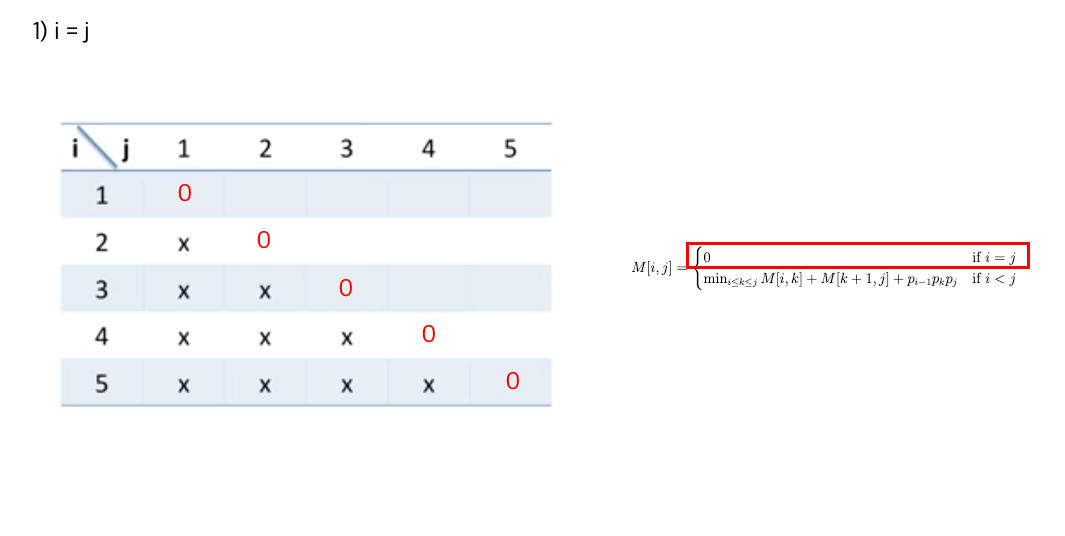
\includegraphics[width=\linewidth]{images/worksheet_3_solution_2.png}
                    \end{center}

                    \item Fill the table for $i < j$ with a spread of 1

                    \begin{center}
                    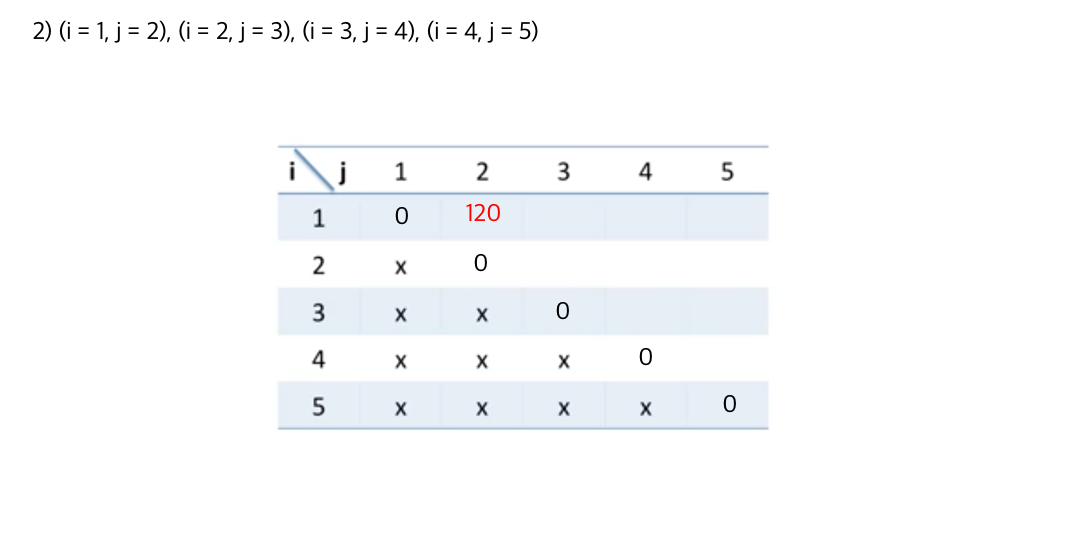
\includegraphics[width=\linewidth]{images/worksheet_3_solution_3.png}
                    \end{center}

                    since

                    \begin{itemize}
                        \item $i = 1, j = 2$

                        \begin{align}
                            M[1,2] &= \min_{1 \leq k \leq 2} (M[1,1] + M[1,2] + p_{i-1}p_kp_j)\\
                            &= \min_{1 \leq k \leq 2} (0 + 0 + p_0p_1p_2)\\
                            &= \min_{1 \leq k \leq 2} (0 + 0 + 4 \cdot 10 \cdot 3)\\
                            &= 120
                        \end{align}

                        where $p_0 = 3$ is from the dimension $3 \times 10$ of $A_1$, $p_k = 10$
                        is from the dimension of $3 \times 10$ of $A_1$.

                        \item $i = 2, j = 3$

                        \begin{align}
                            M[2,3] &= \min_{2 \leq k \leq 3} (M[2,2] + M[3,3] + p_{i-1}p_kp_j)\\
                            &= \min_{2 \leq k \leq 3} (0 + 0 + p_1p_2p_3)\\
                            &= \min_{2 \leq k \leq 3} (0 + 0 + 10 \cdot 3 \cdot 12)\\
                            &= 360
                        \end{align}

                        \item $i = 3, j = 4$

                        \begin{align}
                            M[3,4] &= \min_{3 \leq k \leq 4} (M[3,3] + M[4,4] + p_{i-1}p_kp_j)\\
                            &= \min_{3 \leq k \leq 4} (0 + 0 + p_2p_3p_4)\\
                            &= \min_{3 \leq k \leq 4} (0 + 0 + 3 \cdot 12 \cdot 20)\\
                            &= 720
                        \end{align}

                        \item $i = 4, j = 5$

                        \begin{align}
                            M[4,5] &= \min_{4 \leq k \leq 5} (M[4,4] + M[5,5] + p_{i-1}p_kp_j)\\
                            &= \min_{4 \leq k \leq 5} (0 + 0 + p_3p_4p_5)\\
                            &= \min_{4 \leq k \leq 5} (0 + 0 + 12 \cdot 20 \cdot 7)\\
                            &= 1680
                        \end{align}
                    \end{itemize}

                    \item Repeat 2 with the increased value of spread

                    \begin{center}
                    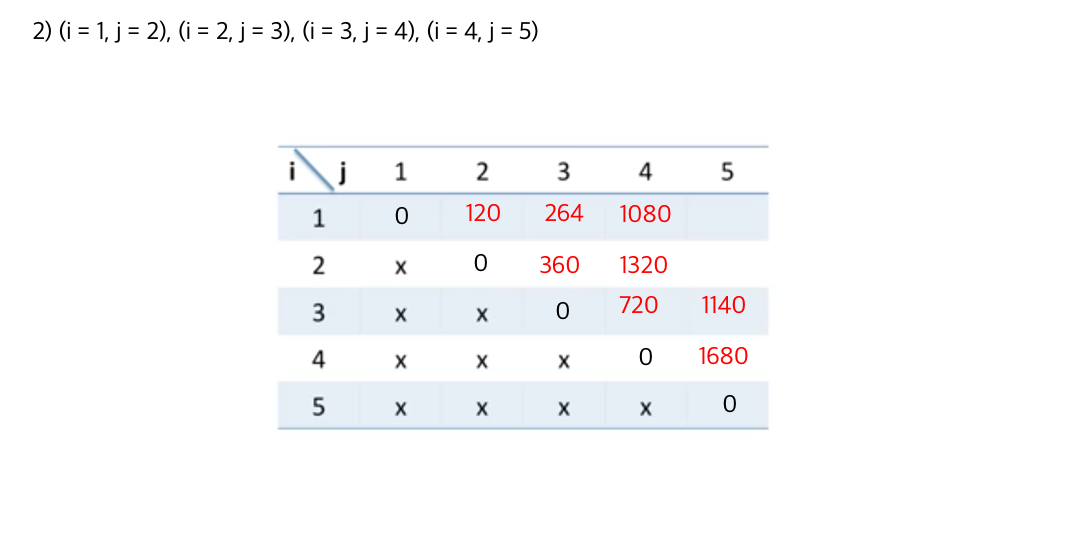
\includegraphics[width=\linewidth]{images/worksheet_3_solution_4.png}
                    \end{center}

                    \begin{itemize}
                        \item $i = 1, j = 3$

                        \bigskip

                        \underline{$k = 1$}

                        \begin{align}
                            M[1,3] &= M[1,1] + M[2,3] + p_{i-1}p_kp_j\\
                            &= 0 + 360 + p_0p_1p_3\\
                            &= 0 + 360 + 4 \cdot 10 \cdot 12\\
                            &= 0 + 360 + 480\\
                            &= 840
                        \end{align}

                        \bigskip

                        \underline{$k = 2$}

                        \begin{align}
                            M[1,3] &= M[1,2] + M[3,3] + p_{i-1}p_kp_j\\
                            &= 120 + 0 + p_0p_2p_3\\
                            &= 120 + 0 + 4 \cdot 10 \cdot 12\\
                            &= 120 + 0 + 144\\
                            &= 264
                        \end{align}

                        \bigskip

                        Thus, $\min_{1 \leq k \leq 3} M[1,3] = 264$.

                        \item $i = 2, j = 4$

                        \bigskip

                        \underline{$k = 2$}

                        \begin{align}
                            M[2,4] &= M[2,2] + M[3,4] + p_{i-1}p_kp_j\\
                            &= 0 + 720 + p_1p_2p_4\\
                            &= 0 + 720 + 10 \cdot 3 \cdot 20\\
                            &= 0 + 720 + 600\\
                            &= 1320
                        \end{align}

                        \bigskip

                        \underline{$k = 3$}

                        \begin{align}
                            M[2,4] &= M[2,2] + M[3,4] + p_{i-1}p_kp_j\\
                            &= 360 + 0 + p_1p_3p_4\\
                            &= 360 + 0 + 10 \cdot 12 \cdot 20\\
                            &= 360 + 0 + 2400\\
                            &= 2760
                        \end{align}

                        \bigskip

                        Thus, $\min_{2 \leq k \leq 4} M[2,4] = 1320$.

                        \item $i = 3, j = 5$

                        \bigskip

                        \underline{$k = 3$}

                        \begin{align}
                            M[3,5] &= M[3,3] + M[3,5] + p_{i-1}p_kp_j\\
                            &= 0 + 1680 + p_2p_3p_5\\
                            &= 0 + 1680 + 3 \cdot 12 \cdot 7\\
                            &= 0 + 1680 + 252\\
                            &= 1932
                        \end{align}

                        \bigskip

                        \underline{$k = 4$}

                        \begin{align}
                            M[3,5] &= M[3,4] + M[5,5] + p_{i-1}p_kp_j\\
                            &= 720 + 0 + p_2p_4p_5\\
                            &= 720 + 0 + 3 \cdot 20 \cdot 7\\
                            &= 720 + 420\\
                            &= 1140
                        \end{align}

                        \bigskip

                        Thus, $\min_{3 \leq k \leq 5} M[3,5] = 1140$.


                        \item $i = 2, j = 5$

                        \bigskip

                        \underline{$k = 2$}

                        \begin{align}
                            M[2,5] &= M[2,2] + M[3,5] + p_{i-1}p_kp_j\\
                            &= 0 + 1140 + p_1p_2p_5\\
                            &= 0 + 1140 + 10 \cdot 3 \cdot 7\\
                            &= 0 + 1140 + 210\\
                            &= 1350
                        \end{align}

                        \bigskip

                        \underline{$k = 2$}

                        \begin{align}
                            M[1,4] &= M[1,2] + M[3,4] + p_{i-1}p_kp_j\\
                            &= 120 + 720 + p_0p_2p_4\\
                            &= 120 + 720 + 4 \cdot 3 \cdot 20\\
                            &= 840 + 240\\
                            &= 1080
                        \end{align}

                        \bigskip

                        \underline{$k = 3$}

                        \begin{align}
                            M[1,4] &= M[1,3] + M[4,4] + p_{i-1}p_kp_j\\
                            &= 264 + 0 + p_0p_3p_4\\
                            &= 264 + 0 + 4 \cdot 12 \cdot 20\\
                            &= 264 + 960\\
                            &= 1254
                        \end{align}

                        \bigskip

                        Thus, $\min_{1 \leq k \leq 4} M[1,4] = 1080$.

                    \end{itemize}


                \end{enumerate}

                \item \textbf{Constructing the Optimal Solution}
            \end{enumerate}
        \end{itemize}

        \bigskip

        \underline{\textbf{References:}}

        \bigskip

        \begin{enumerate}[1)]
            \item
        \end{enumerate}
    \end{itemize}
\end{enumerate}

\end{document}